\documentclass{article}
\usepackage{graphicx}
\graphicspath{{images/}}
\usepackage{hyperref}
\title{TP 4A - Génie Logiciel
Programme Java intégrant modélisation UML, versionning (git)
et tests unitaires (Junit)
}
\author{Mathis Vaugeois - Tanguy Mrc - Faustine Guillou}
\date{January 2023}

\begin{document}

\maketitle

\section*{Sommaire}

\section{Introduction}

\subsection{Context}

\subsection{Git}

\section{Cahier des charges}

\begin{figure}
    \centering
    \includegraphics[width=0.75\textwidth]{diagrammeClasse}
    \caption{A nice plot.}
    \label{fig:mesh1}
\end{figure}

As you can see in figure \ref{fig:mesh1}, the function grows near the origin. This example is on page \pageref{fig:mesh1}.

\section{Code de départ}

\section{Développement}

\section*{Référence}
\url{https://github.com/mathisvaugeois/TPBank-GenieLogiciel}

\end{document}